%!TEX root = mb.tex


\section{Introduction}\label{sec:intro}


    Network processing appliances (``middleboxes'') such as firewalls, NATs, proxies, and intrusion detection systems are crucial components of modern networks~\cite{aplomb,darksideofthemiddle,morley-paper}. 
     In recent trends, more and more organizations are {\it outsourcing} their network processing, either to cloud providers~\cite{aplomb, aryaka, zscalar} or to Interet service providers~\cite{attddos,comcastparentalfiltering}. 
     Network Functions Virtualization (NFV)~\cite{nfv}, which proposes moving network appliances from hardware deployments to virtualized software deployments, makes this move increasingly attractive to service providers who can offer virtualized network functions in a similar fashion to how cloud providers support virtual servers and storage.
     For enterprise clients, this strategy promises to reduce costs, decrease the burden of managing and configuring these devices, and provide redundant resources for elasticity and fault tolerance~\cite{aplomb}.
   
   Nevertheless, outsourcing middleboxes to a third party service provider brings a new and important challenge: the confidentiality of client traffic. In order to be able to process and examine the traffic of an organization, the service provider  receives  the traffic {\em unencrypted}.  Consequently, the service provider has access to potentially sensitive packet payloads,  IP addresses, and ports revealing confidential information about the organization. This situation is worrisome considering the increasing prevalence data breaches by cloud employees or hackers gaining access to clouds~\cite{PrivacyRecords, more, more, makeitsoundsuperscary}.
   Hence, the question we ask in this paper is, can we enable a third party to perform traffic processing for an enterprise, {\em without seeing the enterprise's traffic}?
   
   
    We design and build \sys (read ``embark"), the first system that enables a service provider to offer a wide range of middleboxes  while maintaining the confidentiality of the traffic. \sys provides these guarantees even against attackers who gain access to {\em all} the data at the cloud.  
    %\sys's name concatenates the words MB (middlebox) and Ark (protection). 
  In traditional outsourcing configurations, an enterprise uses an outsourcing gateway which encrypts traffic -- both payloads and headers -- and then tunnels the data to a service provider~\cite{aplomb}.
  The service provider then decrypts the traffic before performing traffic processing.
  With \sys, this configuration is changed only by removing the requirement that the traffic first be decrypted.
    Per-packet operations at the middlebox remain entirely unchanged: they treat encrypted packets and rules just as they treat plaintext packets and rules.
   Consequently there is {\it no overhead} in forwarding rates for most middleboxes at the service provider.

   Designing \sys required overcoming two critical challenges: (1) achieving sufficient generality -- so as to support the wide range of operations performed by middleboxes today, and (2) achieving accepable performance for practical deployments. 
    Typically, the more general operations a functional or homomorphic encryption scheme supports, the more expensive it is in terms of performance overheads -- requiring days of computation for simple operations under the most expressive schemes~\cite{fhe, blah, blah}.
    However, even more restricted schemes to date still do not provide practical overheads for typical use -- for example, BlindBox~\cite{blindbox} a system which enables string-matching for deep-packet inspection (not middleboxes in general) imposes a 97 second overhead on every client connection.
    This system -- the only other system to perform privacy preserving packet processing -- is both more limited in capabilities than \sys, while imposing unacceptable overheads.

    \sys achieves both generality with practical performance through a combination of cryptographic and systems innovations.
    \sys relies on two forms of computational encryption: {\it keyword match}, a form of searchable encryption~\cite{blindbox}, and {\it RangeMatch}.
    RangeMatch is a new encryption scheme we designed for \sys in order to enable the provider to perform prefix matching (\eg{}, if an IP address is in the subdomain 56.24.67.0/16) or port range detection (\eg., if a port is in the range 1000-2000), which are common actions performed by middleboxes such as firewalls. 
    Using just these two encryption schemes, we implemented a wide range of encrypted security appliances -- such as a firewall and an intrusion detection system -- as well as performance-enhancing appliances, including  a web proxy and a load balancer. 
    We present a full list of the appliances \sys supports, and how it supports them, in \S\ref{sec:appliances}.

    We designed {\it RangeMatch} because no existing system provided the computational expressiveness, performance properties, and the privacy properties we desired for \sys.
    Of existing cryptographic schemes, OPE~\cite{cryptdb} is the closest relative of {\it RangeMatch}; however, it is four orders of magnitude slower than {\it RangeMatch} and leaks unnecessary information to the cloud provider.
    Where {\em RangeMatch} only reveals whether or not a value lies within a pre-determined range, OPE reveals the total ordering among all encrypted values, whether they lie within a range or not.
    We discuss the {\em RangeMatch} scheme in \S\ref{sec:rangematch}.

    
\newcounter{theapp} \setcounter{theapp}{0}  
\newcommand{\capp}{\refstepcounter{theapp}\arabic{theapp}}

% 2nd fig/1st fig = 1.12 ratio
\begin{figure*}[t!]
\centering
\subfigure[Enterprise to external site communication]{
  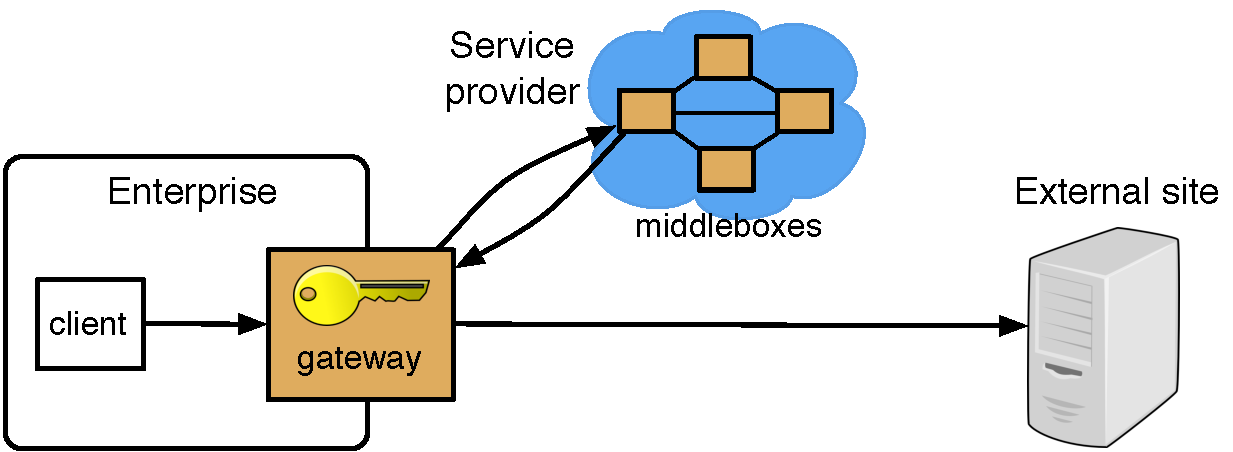
\includegraphics[width=2.8in]{fig/model_1.pdf}
  \label{fig:model1} }
%
\hfill  
\subfigure[Enterprise to enterprise communication]{
   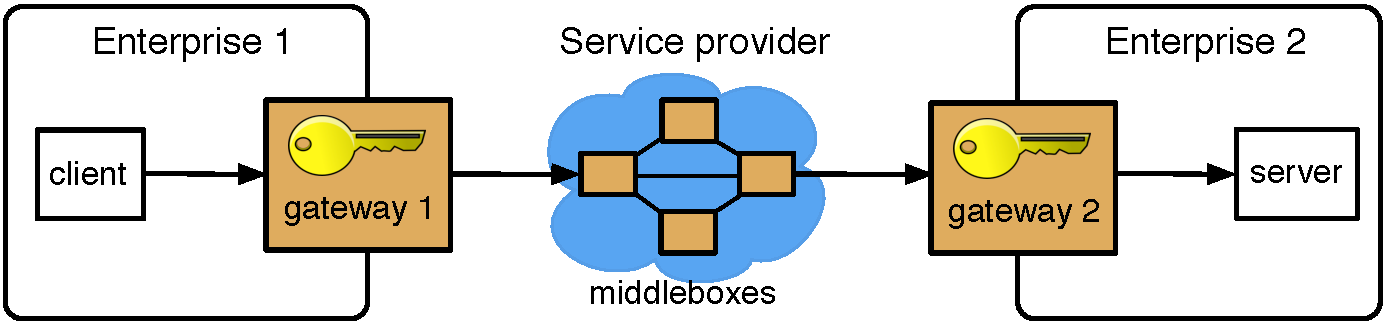
\includegraphics[width=3.2in]{fig/model_2.pdf}
     \label{fig:model2}}
     
     %
\caption{System architecture. Aplomb and NFV system setup with \sys encryption  at the gateway. The arrows indicate traffic from the client to the server; the response traffic follows the reverse direction. \label{fig:sys-overview}}
\end{figure*}


  From a systems perspective, \sys achieves low overheads by being deliberate in how and where it introduces overheads due to encryption. 
  These costs are divided between the service provider, and the outsourcing gateway installed at the enterprise.
  
  At the service provider, \sys keeps packet formats unchanged: an encrypted IP packet is structured just as a normal IP packet, with each field (e.g., source address) containing an encrypted value of that field. 
  Structuring packets in this way, combined with {\it KeywordMatch} and {\it RangeMatch}, allows most middleboxes to remain completely unmodified on the dataplane, importantly, taking advantage of highly-efficient packet classification algorithms~\cite{somethingclassification--chang?} as already implemented.
  Consequently, forwarding rates at the service provider are unchanged for these middleboxes; furthermore, the two middleboxes which do require dataplane modifications -- web proxies and intrusion detection systems -- have similarly low overheads in processing rates.
  %Instead, the primary costs from \sys come in performing rule updates.
  %Inserting or deleting rules to an active system are more expensive than under an unencrypted scheme; because these tasks are rare and typically operate under human time scales, these overheads are more acceptable than dataplane overheads.
  We discuss deployment at the service provider, and how middleboxes are modified to support \sys, in \S\ref{sec:middleboxes}.

  At the enterprise, it is important to keep the outsourcing gateway simple and cost-effective to deploy.
  Were the gateway to be expensive, it would defeat the purpose of clients outsourcing in the first place! 
  To achieve this, we ensure that the gateway keeps {\it no per-connection state}, that it only perform {\it inexpensive per-packet operations}, and that it be {\it parallelizable}.
  We discuss the design and implementation of the gateway in~\S\ref{sec:gateway}.


We implemented and evaluated \sys. As mentioned, we support all applications fit in the outsourcing model, as surveyed in~\cite{aplomb} -- any appliance which it outsourced today can also be outsourced using \sys.
Further, \sys imposes very negligible throughput overheads at the service provider: for example, a single-core firewall operating over encrypted data achieves 9.8Gbps, equal to the same firewall over unencrypted data.
Our enterprise gateway can tunnel traffic at 1.5 Gbps on a single core;  our 8 core server can transmit \sys encrypted data at up to the full 10Gbps line rate of its network interface.
